\documentclass[runningheads]{llncs}

\usepackage[T1]{fontenc}
\usepackage{graphicx}
\usepackage{booktabs}
\usepackage{amsmath}
\usepackage{amssymb}
\usepackage{multirow}
\usepackage{url}
\usepackage{array}
\setlength{\tabcolsep}{6.5pt}

\graphicspath{{../reports/figures/}{reports/figures/}{figures/}{./}}

\title{ReviewGuard: Filtering Coordinated Review Spam via Reliability Weighting}
\titlerunning{ReviewGuard}

\author{Anonymous}
\authorrunning{Anonymous}
\institute{Anonymous Institution}

\begin{document}
\maketitle

\begin{abstract}
App-store reviews influence both user choices and product feedback analysis, creating incentives for commercial or reputational manipulation through coordinated review spam. In this paper, we study review spam filtering for rating-derived sentiment (negative, neutral, and positive) proportion recovery: the goal is to reduce distortion in sentiment proportions computed from a review stream affected by coordinated spam. We propose ReviewGuard to address a practical gap in app-review analytics: coordinated spam can distort sentiment summaries even when individual reviews appear plausible, and many app-review exports lack reviewer graphs or human-verified spam labels. Rather than making a brittle keep-or-delete decision, ReviewGuard estimates how much each review should contribute to the final sentiment proportions. This design reduces the collective influence of coordinated review groups while preserving individually consistent reviews and keeping the original review records unchanged. ReviewGuard supports two settings: its base filtering mode reports weighted sentiment proportions when no verified clean sample is available, and its verified-sample calibration mode adjusts the recovered sentiment proportions when a small verified clean sample is available. We evaluate recovery with total variation distance (TVD), which measures the discrepancy between recovered and pre-injection reference proportions. Averaged over the five evaluated attack ratios, ReviewGuard reduces mean TVD from 0.1121 without filtering to 0.0138, an 87.7\% relative reduction. In an optimistic simulated verified-sample calibration setting, TVD further decreases to 0.0038; this result is reported separately because it uses simulated trusted-sample information.
\keywords{App reviews \and Review spam \and Sentiment proportion recovery \and Reliability weighting \and Noise-aware aggregation}
\end{abstract}

\section{Introduction}

App reviews are a direct and high-volume signal for user choices and product feedback analysis. Product teams use them to track user satisfaction, detect regressions after releases, compare app versions, and prioritize engineering work. App-review analytics often analyzes sentiment and feedback categories in review text \cite{guzman2014users,maalej2016automatic}. In this work, we derive the sentiment summary from star ratings because ratings are consistently available in app-store exports and directly determine public rating summaries. This avoids relying only on text classifiers, whose outputs can vary with training data, model architecture, and decision thresholds.

This summary assumes that the observed review stream represents real user experience. In practice, the assumption can fail when app reviews contain \emph{coordinated spam}, such as duplicated or semantically similar negative reviews and bursts of low ratings that share patterns in posting time, review text, star rating, or app version. Since coordinated spam affects the summary through shared behavior across multiple reviews rather than through a single review alone, we use \emph{cohort} to denote a candidate set of reviews that share such observable patterns, for example similar text posted within a short period, concentrated low ratings, or repeated complaints tied to the same app version. If such cohorts are treated as unfiltered user feedback, they can artificially inflate negative or positive review proportions and misrepresent the sentiment distribution used for user choice and product analysis.

Figure~\ref{fig:intro_problem} gives an illustrative example of this distortion. Starting from 100 reviews with 25 negative, 5 neutral, and 70 positive ratings, injecting 20 coordinated negative reviews changes the observed stream to 45 negative, 5 neutral, and 70 positive reviews, increasing the apparent negative proportion from 25.0\% to 37.5\%. A no-defense summary directly reflects this polluted stream. A hard-deletion baseline tries to remove suspicious reviews but can also remove legitimate complaints. ReviewGuard instead keeps all review records and reduces the contribution weights of coordinated suspicious reviews, moving the weighted sentiment estimate closer to the pre-injection reference.

\begin{figure}[h]
\centering
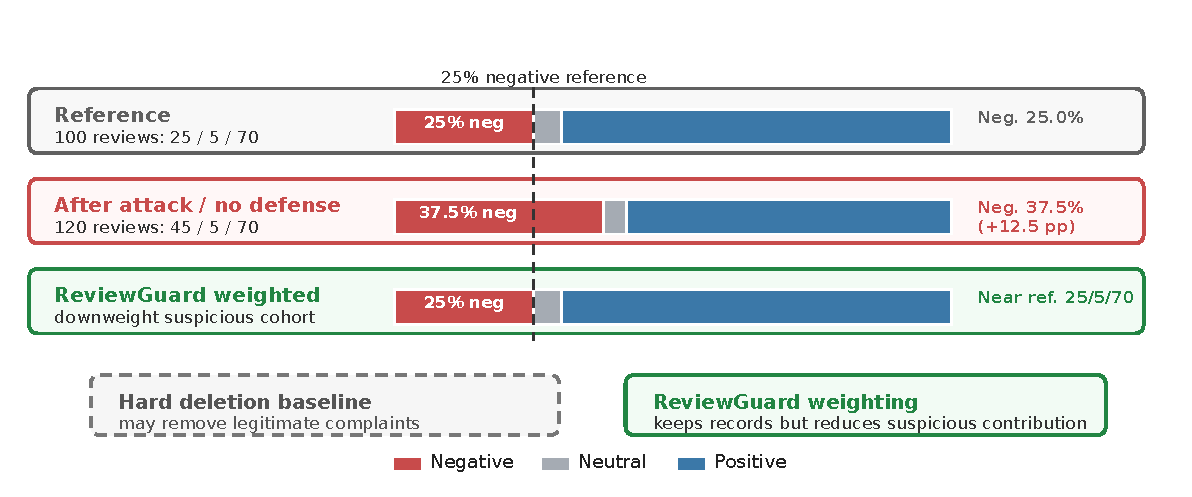
\includegraphics[width=\linewidth]{intro_problem_baseline_example.pdf}
\caption{Illustrative example of coordinated review-spam distortion and weighting-based repair. Injecting 20 similar negative reviews into a 100-review reference stream shifts the observed sentiment distribution; hard deletion can be coarse, whereas ReviewGuard keeps reviews and reduces the contribution of suspicious coordinated reviews.}
\label{fig:intro_problem}
\end{figure}

Relevant work spans sentiment analysis and app-review mining \cite{devlin2019bert,guzman2014users,maalej2016automatic}, opinion-spam detection \cite{mukherjee2013spotting,li2014spotting,dou2020caregnn,liu2021pcgnn,wu2023splitgnn}, and noisy-label learning \cite{han2018coteaching,li2020dividemix,liu2020early,northcutt2021confident}. However, these lines do not directly address coordinated distortion of rating-derived sentiment proportions when app-store exports lack reviewer graphs and verified spam labels. We therefore define \emph{review spam filtering for rating-derived sentiment proportion recovery} using only review text, rating, timestamp, and app version. Because hard removal is too coarse when coordinated patterns can coexist with plausible feedback, ReviewGuard retains every record and estimates its contribution to the recovered proportions. ReviewGuard is not intended to assign definitive spam labels to individual reviews; instead, it reduces aggregate sentiment distortion while preserving review records for inspection.

ReviewGuard combines group evidence from posting time, text, rating, version, and semantic similarity with review-level text--rating consistency. Their multiplicative fusion requires both reliability scores to remain high, so loss evidence cannot reverse a reduction imposed by group evidence. The base mode returns weighted proportions without verified clean data; when a small verified clean sample is available, the calibrated mode adjusts residual class bias.

Our contributions are:
\begin{itemize}
    \item We define coordinated review spam filtering as rating-derived sentiment proportion recovery for app-review streams.
    \item We propose ReviewGuard, which estimates each review's contribution to the recovered sentiment proportions by combining group evidence with loss-based consistency evidence.
    \item We evaluate ReviewGuard in two deployment settings: base filtering without verified clean samples and verified-sample calibration with a small verified clean sample.
    \item We evaluate ReviewGuard with controlled review spam injections, multi-stream evaluation, attack-type analysis, false-positive diagnostics, stress tests, scaling analysis, and ablation.
\end{itemize}

\section{Related Work}

\paragraph{App review mining and sentiment analysis.}
App-review mining motivates this work because reviews are used to summarize user satisfaction, release regressions, and developer-relevant feedback. Prior studies show that app-store reviews contain requirements and quality signals and support sentiment or feedback classification \cite{pagano2013user,guzman2014users,maalej2016automatic,hadi2023evaluating,mukherjee2020security}. General sentiment models, including pretrained language models such as BERT, further improve review classification \cite{devlin2019bert}. These studies mainly improve review understanding, whereas ReviewGuard asks whether rating-derived sentiment proportions remain reliable when coordinated spam changes the observed review stream.

\paragraph{Review spam and anomaly detection.}
Once sentiment proportions become the target output, the next question is whether the observed reviews should be trusted as user feedback. Opinion-spam and fraud-detection studies analyze duplicate reviews, group spam, and fake-review spotting \cite{jindal2008opinion,mukherjee2013spotting,li2014spotting}. Recent detectors often exploit graph structure or benchmark labels \cite{rayana2015collective,dou2020caregnn,liu2021pcgnn,wu2023splitgnn}, but many app-store exports lack reviewer-product relations and verified spam labels. ReviewGuard therefore estimates group evidence from observable review fields while keeping rating-derived sentiment proportion recovery as the primary app-review task.

\paragraph{Learning with noisy labels.}
Group evidence alone is not sufficient, because real product incidents can also create concentrated low-rating reviews. Noisy-label learning uses small-loss selection, loss mixtures, or label-error estimation to identify examples that fit patterns learned from the rest of the data \cite{han2018coteaching,wei2020jocor,li2020dividemix,tan2021colearning,wei2021noisylabels,song2022survey,northcutt2021confident}. Such loss behavior provides complementary review-level consistency evidence, but independent noisy-label assumptions do not capture the collective effect of coordinated spam on sentiment proportions. ReviewGuard therefore combines loss-based consistency with group evidence rather than basing review contributions on either signal alone.

\paragraph{Trusted data and calibration.}
After group evidence and loss-based consistency estimate review contributions, a remaining practical issue is calibration under different data availability conditions. Small trusted datasets can improve learning under severe label noise \cite{hendrycks2018trusted}. ReviewGuard uses the same principle for proportion recovery: it operates in base filtering mode without verified clean samples and calibrates recovered sentiment proportions when limited verified clean data are available.

\section{Methodology}

\subsection{System Overview and Task Definition}

ReviewGuard has five modules, shown in Fig.~\ref{fig:reviewguard_workflow}. The \emph{group-reliability module} \(\mathcal{G}\) converts cohort-level temporal, textual, rating, version, and semantic evidence into a score \(c_i\) for each review. In parallel, the \emph{loss-reliability module} \(\mathcal{L}\) uses out-of-fold text-to-rating-label prediction to obtain a review-level consistency score \(u_i\). The \emph{fusion module} \(\mathcal{F}\) combines these complementary scores into a base contribution weight \(w_i\). When independently verified clean reviews are available, the optional \emph{calibration module} \(\mathcal{C}\) adjusts the base weights by class; otherwise the base weights are used unchanged. Finally, the \emph{aggregation module} \(\mathcal{A}\) converts the resulting review weights into recovered sentiment proportions. Sections~3.2--3.4 define these modules and their parameters.

Formally, the observed review stream is
\[
D=\{d_i\}_{i=1}^{n}, \qquad d_i=(x_i,s_i,t_i,v_i),
\]
where \(x_i\), \(s_i\), \(t_i\), and \(v_i\) denote text, star rating, timestamp, and app version, respectively. A fixed rating map \(g\) gives \(y_i=g(s_i)\in\mathcal{Y}\), with \(\mathcal{Y}=\{\mathrm{neg},\mathrm{neu},\mathrm{pos}\}\). We use \(\mathbf{x}=(x_i)_{i=1}^{n}\) and \(\mathbf{y}=(y_i)_{i=1}^{n}\) for the text and label sequences.

We collect the group- and loss-module parameters as
\[
\Theta_G=\{\phi,\kappa,K_c,B,\lambda_{low},\boldsymbol{\beta}_0,
\tau,\alpha,\omega\},
\qquad
\Theta_L=\{K,\rho\}.
\]

The module-level data flow is
\begin{equation}
\mathbf{c}=\mathcal{G}_{\Theta_G}(D), \qquad
\mathbf{u}=\mathcal{L}_{\Theta_L}(\mathbf{x},\mathbf{y}), \qquad
\mathbf{w}=\mathcal{F}_{\delta}(\mathbf{c},\mathbf{u}),
\label{eq:reviewguard_base_flow}
\end{equation}
where \(\mathbf{c}=(c_i)_{i=1}^{n}\), \(\mathbf{u}=(u_i)_{i=1}^{n}\), and \(\mathbf{w}=(w_i)_{i=1}^{n}\). Here \(c_i\) measures reliability under group evidence, \(u_i\) measures text--rating consistency, and \(w_i\) is their fused contribution weight. These quantities are intermediate outputs rather than observed inputs.

Let \(D^{clean}\subseteq D\) be the unknown subset not belonging to coordinated spam. In the calibrated setting, \(T\subseteq D^{clean}\) is a small independently verified subset with the same schema and rating map as \(D\); \(T=\varnothing\) denotes the base setting. The final weight vector is
\begin{equation}
\bar{\mathbf{w}}=
\begin{cases}
\mathbf{w}, & T=\varnothing,\\
\mathcal{C}_{\epsilon,\delta}(T,\mathbf{y},\mathbf{w}), & T\neq\varnothing.
\end{cases}
\label{eq:reviewguard_modes}
\end{equation}
The aggregation module then returns \(\hat{\mathbf{p}}=\mathcal{A}(\mathbf{y},\bar{\mathbf{w}})\), whose component for sentiment class \(y\in\mathcal{Y}\) is
\begin{equation}
\hat{p}_y=
\frac{\sum_{i=1}^{n}\bar{w}_i\mathbb{1}[y_i=y]}
{\sum_{i=1}^{n}\bar{w}_i}.
\label{eq:weighted_aggregation_overview}
\end{equation}

The system returns
\begin{equation}
\boxed{
\operatorname{ReviewGuard}(D;T)
=\left(D^{RG},\hat{\mathbf{p}}\right)
},
\label{eq:reviewguard_output}
\end{equation}
where \(D^{RG}=\{(d_i,y_i,\bar{w}_i)\}_{i=1}^{n}\) is the weighted review table. Thus, the inputs are \(D\) and optional \(T\), while the outputs are \(D^{RG}\) and \(\hat{\mathbf{p}}\). ReviewGuard retains every original record; a smaller \(\bar{w}_i\) changes only review \(i\)'s contribution to the aggregate.

For evaluation, let \(\mathbf{p}^{clean}\) denote the rating-derived sentiment distribution of \(D^{clean}\), with
\[
p_y^{clean}
=\frac{1}{|D^{clean}|}
\sum_{d_i\in D^{clean}}\mathbb{1}[y_i=y],
\qquad y\in\mathcal{Y}.
\]
The discrepancy between the recovered and clean distributions is measured by total variation distance:
\[
\mathrm{TVD}(\mathbf{p}^{clean},\hat{\mathbf{p}})
=\frac{1}{2}\sum_{y\in\mathcal{Y}}
\left|p_y^{clean}-\hat{p}_y\right|.
\]
TVD is available only when an appropriate evaluation reference is known; it is not a deployment output. Figure~\ref{fig:reviewguard_workflow} summarizes the same module order as Eqs.~\ref{eq:reviewguard_base_flow}--\ref{eq:weighted_aggregation_overview}.

\begin{figure}[t]
\centering
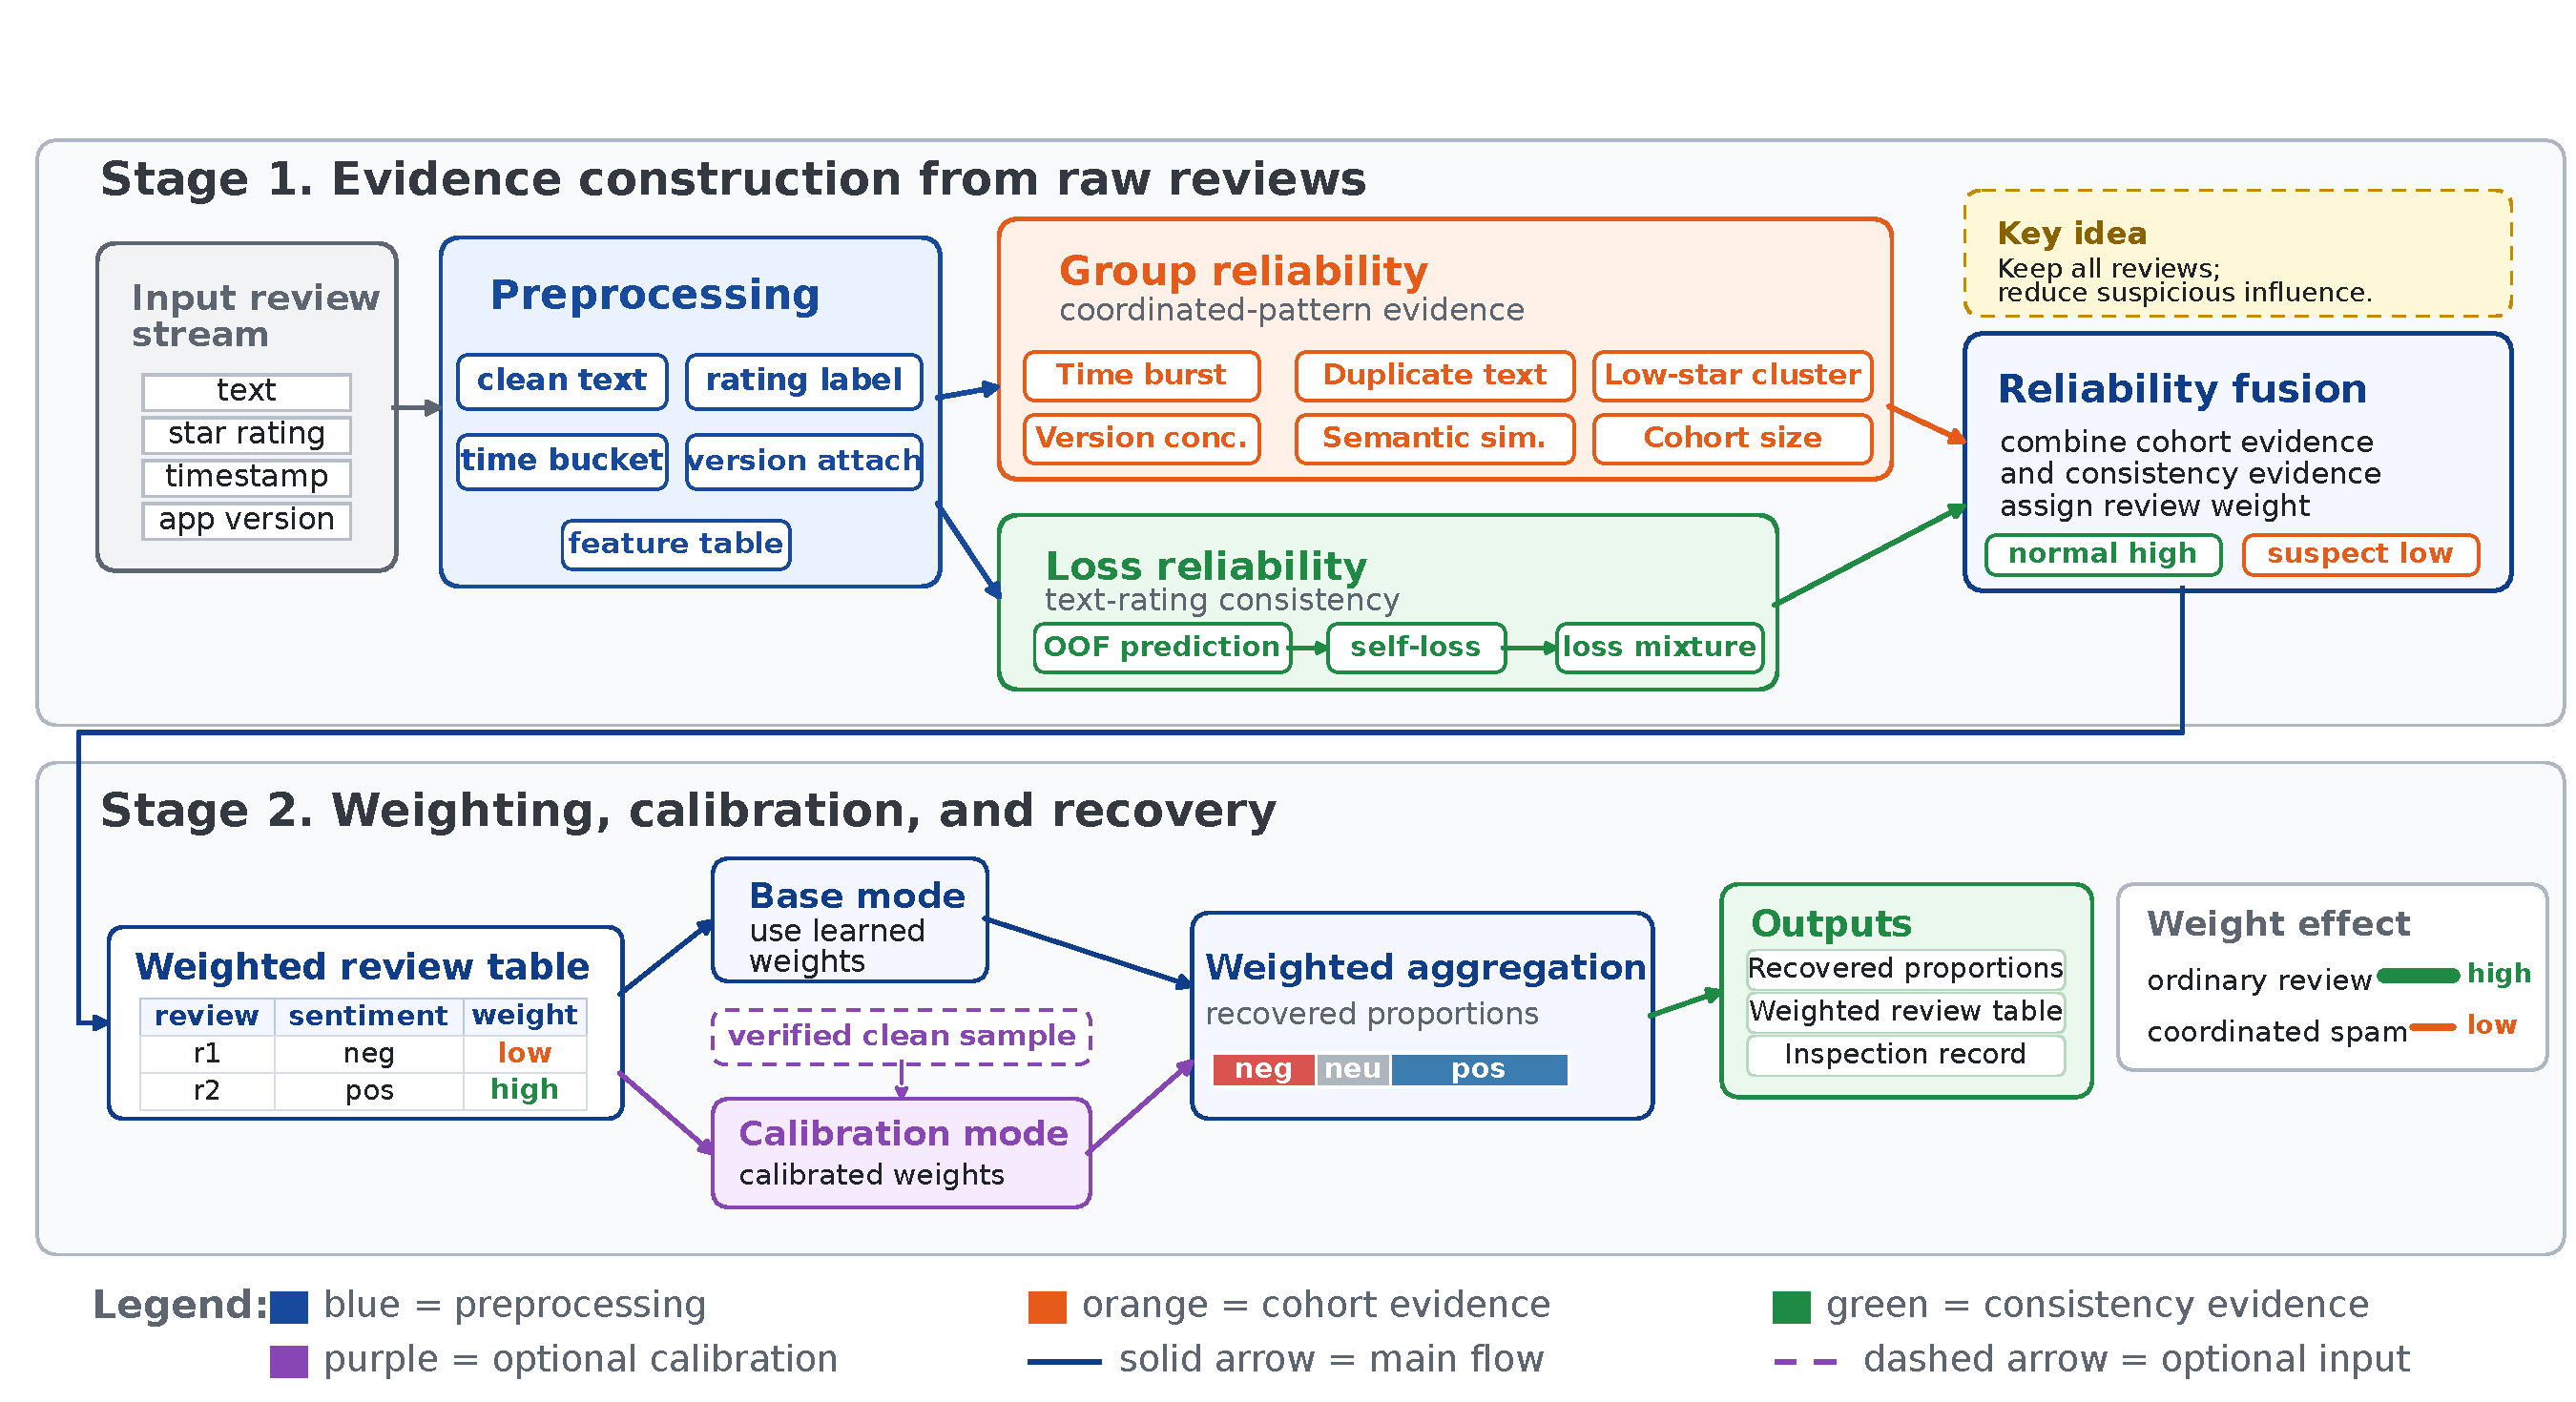
\includegraphics[width=\linewidth]{reviewguard_workflow_flow_only.pdf}
\caption{ReviewGuard method flow. The observed review stream is processed by parallel group- and loss-reliability modules, followed by reliability fusion, optional verified-sample calibration, and weighted sentiment-proportion aggregation. Fixed contribution-weight bounds are omitted for readability and defined in Section~3.4.}
\label{fig:reviewguard_workflow}
\end{figure}

\subsection{Group-Reliability Function}

\paragraph{Candidate cohort construction.}
The group-reliability function \(\mathcal{G}_{\Theta_G}\) first forms candidate cohorts. The text-representation function \(\phi\) maps each review text to a feature vector \(\mathbf{e}_i=\phi(x_i)\). The clustering function \(\kappa\) assigns review \(i\) a cluster identifier \(a_i=\kappa(\mathbf{e}_i;K_c)\). We then define the cohort containing review \(i\) as \(C(i)=\{j:a_j=a_i\}\). The choices of \(\phi\) and \(\kappa\), together with \(K_c\), are specified in the experimental setup.

\paragraph{Cohort-feature extraction.}
To define the data flow, let \(b_i=B(t_i)\) be the posting-time bucket assigned by a chosen time-bucketing function \(B\), and let \(\tilde{x}_i\) denote normalized text obtained by lowercasing, trimming, and collapsing repeated whitespace. For any scalar sequence \(\boldsymbol{\xi}=(\xi_i)_{i=1}^{n}\), define the component-wise min--max operator
\[
[\operatorname{MM}(\boldsymbol{\xi})]_i=
\begin{cases}
\dfrac{\xi_i-\min_j \xi_j}{\max_j \xi_j-\min_j \xi_j},
& \max_j \xi_j>\min_j \xi_j,\\[2mm]
0, & \text{otherwise}.
\end{cases}
\]
It maps a non-constant sequence to \([0,1]\) and a constant sequence to zero. Define the raw feature sequences by \(\xi_i^{burst}=\max(0,z_{b_i})\), \(\xi_i^{dup}=\log(1+\#\{j:\tilde{x}_j=\tilde{x}_i\})\), \(\xi_i^{sem}=\cos(\mathbf{e}_i,\boldsymbol{\mu}_{C(i)})\), and \(\xi_i^{size}=\log(1+|C(i)|)\). ReviewGuard computes six cohort-evidence features bounded in \([0,1]\):
\begin{itemize}
    \item \(h_i^{burst}=[\operatorname{MM}(\boldsymbol{\xi}^{burst})]_i\), where \(z_b\) is the z-score of the number of reviews posted in time bucket \(b\);
    \item \(h_i^{dup}=[\operatorname{MM}(\boldsymbol{\xi}^{dup})]_i\), measuring exact duplicates after text normalization;
    \item \(h_i^{low}=|C(i)|^{-1}\sum_{j\in C(i)}\mathbb{1}[s_j\le \lambda_{low}]\), the fraction of low-star reviews in the cohort, where \(\lambda_{low}\) is the low-rating threshold;
    \item \(h_i^{ver}=\max_v |C(i)|^{-1}\sum_{j\in C(i)}\mathbb{1}[v_j=v]\), the dominant app-version share in the cohort;
    \item \(h_i^{sem}=[\operatorname{MM}(\boldsymbol{\xi}^{sem})]_i\), where \(\boldsymbol{\mu}_{C(i)}\) is the centroid of cohort \(C(i)\);
    \item \(h_i^{size}=[\operatorname{MM}(\boldsymbol{\xi}^{size})]_i\), the normalized log cohort size.
\end{itemize}

\paragraph{Risk-to-reliability mapping.}
Let \(i\) index a review in the observed stream \(D\), and let
\[
\mathbf{h}_i=[h_i^{burst},h_i^{dup},h_i^{low},h_i^{ver},h_i^{sem},h_i^{size}]
\]
denote the six cohort-feature scores for that review. We write \(h_{ij}\) for the \(j\)-th entry of \(\mathbf{h}_i\), where \(j\) ranges over burst, duplicate-text, low-rating, version, semantic, and size evidence. ReviewGuard computes the cohort-risk score of review \(i\) as
\[
r_i(\boldsymbol{\beta})=\sum_{j=1}^{6}\beta_j h_{ij},
\qquad
\beta_j\ge 0,\quad \sum_{j=1}^{6}\beta_j=1 .
\]
The non-negative sum-to-one constraint makes \(r_i(\boldsymbol{\beta})\) a weighted average of cohort evidence rather than an unconstrained score. ReviewGuard uses the default cohort-feature weight vector \(\boldsymbol{\beta}_0\), specified in the experimental settings. This vector is fixed for base filtering; the experiments separately examine alternative non-negative weight vectors.

ReviewGuard maps cohort risk into cohort reliability:
\[
c_i = \omega + (1-\omega)\sigma[-\alpha(r_i(\boldsymbol{\beta}_0)-\tau)],
\]
where \(c_i\in[\omega,1]\) is the cohort reliability score of review \(i\), \(\sigma(z)=1/(1+\exp(-z))\) is the sigmoid function, \(\tau\) is the risk value at which the sigmoid has its maximum slope magnitude, \(\alpha\) controls the slope magnitude around \(\tau\), and \(\omega\) is the lower bound of the cohort reliability score. Larger \(r_i(\boldsymbol{\beta}_0)\) therefore produces smaller \(c_i\), so reviews with stronger cohort evidence contribute less to the recovered sentiment proportions.

The cohort-risk score is decomposable into the six feature contributions \(\beta_{0j}h_{ij}\), corresponding to posting-time, duplicate-text, star-rating, app-version, semantic-similarity, and cohort-size evidence.

\subsection{Loss-Reliability Function}

The loss-reliability function \(\mathcal{L}_{\Theta_L}\) provides review-level evidence complementary to cohort evidence. It estimates whether each review belongs to the low-loss component of the observed loss distribution. We call this module DivideMix-style because it adopts the DivideMix principle of separating low-loss and high-loss examples with a mixture model over per-sample losses \cite{li2020dividemix}; it does not use the full DivideMix semi-supervised co-training procedure. Starting from the same observed stream \(D\), this module converts each review text \(x_i\) into one or more text feature views and uses the rating-derived sentiment label \(y_i\) as the prediction target.

We split \(D\) into \(K\) stratified folds \(\{F_k\}_{k=1}^{K}\), preserving the class proportions of \(\mathcal{Y}\) as much as possible. Here, \(K\) is the number of out-of-fold splits. For each fold \(F_k\), ReviewGuard trains multinomial logistic classifiers on \(D\setminus F_k\) and predicts labels only for reviews in the held-out fold \(F_k\). If multiple text views are used, their held-out probability vectors are averaged. This out-of-fold design prevents the loss of review \(i\) from being computed by a classifier trained on the same review. After all folds are processed, every review has exactly one averaged held-out probability vector, denoted by \(\bar{\mathbf{p}}_i^{OOF}\). The probability assigned to the observed sentiment label is
\[
q_i=\bigl[\bar{\mathbf{p}}_i^{OOF}\bigr]_{y_i},
\]
and the corresponding self-loss is
\[
\ell_i=-\log(q_i).
\]
Using the operator defined above, ReviewGuard computes \(\tilde{\boldsymbol{\ell}}=\operatorname{MM}(\boldsymbol{\ell})\), where \(\boldsymbol{\ell}=(\ell_i)_{i=1}^{n}\). It then fits a two-component Gaussian mixture to \(\{\tilde{\ell}_i\}_{i=1}^{n}\). The component with the smaller mean contains reviews assigned lower out-of-fold negative log-likelihood. The posterior probability of belonging to this component is
\[
\pi_i=P(z_i^{mix}=\mathrm{low}\mid \tilde{\ell}_i),
\]
where \(z_i^{mix}\) is the latent mixture component associated with review \(i\). The posterior \(\pi_i\) is evidence of low-loss consistency, not a verified clean label. ReviewGuard converts it into the loss-based reliability
\[
u_i=\rho+(1-\rho)\pi_i,
\]
where \(\rho\) is a loss-floor parameter that keeps the loss-based reliability above zero.

\subsection{Fusion, Calibration, and Aggregation}

Define \(\operatorname{clip}(a,\delta,1)=\min(1,\max(\delta,a))\). The fusion function \(\mathcal{F}_{\delta}\) combines group reliability and loss-based reliability:
\[
w_i=\operatorname{clip}(c_i u_i,\delta,1).
\]
The unclipped product implements a multiplicative conjunction between the two scores; it does not assume statistical independence. A high \(u_i\) leaves the reduction imposed by \(c_i\) largely unchanged, whereas a low \(u_i\) further reduces the contribution weight. A linear sum could allow one high score to compensate for the other low score, while subtraction does not preserve a direct score interpretation on \([0,1]\). The lower bound \(\delta\) prevents any retained record from receiving a numerically negligible contribution. Unlike hard filtering, weighted aggregation lowers the review's contribution while retaining the original review record for inspection. We empirically compare product, minimum, geometric mean, and linear averaging in Section~4.3, and we report correlations between \(c_i\) and \(u_i\) to quantify the empirical association between the two scores.

Without a verified clean sample, \(\bar{w}_i=w_i\), and the base filtering mode returns
\[
\hat{\mathbf{p}}^{base}=\mathcal{A}(\mathbf{y},\mathbf{w}).
\]
When a verified clean sample \(T\) is available, the calibration function \(\mathcal{C}_{\epsilon,\delta}\) adjusts the base weights to reduce the discrepancy between the weighted sentiment distribution and the sentiment distribution \(\mathbf{p}^{T}\) of \(T\), where
\[
p_y^{T}=\frac{1}{|T|}\sum_{d_i\in T}\mathbb{1}[y_i=y],
\qquad y\in\mathcal{Y}.
\]
Let \(p_y^{T}\) and \(\hat{p}^{base}_y\) denote the respective entries of \(\mathbf{p}^{T}\) and \(\hat{\mathbf{p}}^{base}\) for class \(y\). The class-calibration factor and calibrated review weight are
\[
\gamma_y=\frac{p_y^{T}}{\hat{p}^{base}_y+\epsilon},
\qquad
w_i^{cal}=\operatorname{clip}(\gamma_{y_i}w_i,\delta,1).
\]
Here, \(\epsilon\) is a small constant for numerical stability when a class has near-zero weighted mass. The same fixed bounds are applied after class calibration, so \(w_i^{cal}\in[\delta,1]\). In the calibrated mode, \(\bar{w}_i=w_i^{cal}\), and the final recovered distribution is
\[
\hat{\mathbf{p}}^{cal}
=\mathcal{A}(\mathbf{y},\mathbf{w}^{cal}).
\]
Consequently, the final weight \(\bar{w}_i\) used in the system output of Eq.~\ref{eq:reviewguard_output} is \(w_i\) in base filtering mode and \(w_i^{cal}\) in calibrated mode. In both modes, \(D^{RG}\) retains every original review and appends \(\bar{w}_i\); the corresponding recovered distribution is obtained by applying \(\mathcal{A}\) to the same final weights.

\section{Experiments}

\subsection{Experimental Settings}

\paragraph{Datasets.}
Table~\ref{tab:data_profile} summarizes the datasets and fields used in the experiments. The two review datasets are used for controlled-injection evaluation because they contain the fields required by ReviewGuard: review text, star rating, timestamp, and app version \cite{kaggleUberReviews,kaggleGooglePlayApps}. Ratings are mapped to sentiment categories as negative (1--2 stars), neutral (3 stars), and positive (4--5 stars).

\begin{table}
\centering
\small
\setlength{\tabcolsep}{3.5pt}
\caption{Datasets, effective fields, and label categories used in the experiments.}
\label{tab:data_profile}
\begin{tabular}{@{}>{\raggedright\arraybackslash}p{2.5cm}>{\raggedright\arraybackslash}p{3.9cm}>{\raggedright\arraybackslash}p{2.4cm}>{\raggedright\arraybackslash}p{2.6cm}@{}}
\toprule
Dataset and source & Effective fields & Label categories & Experimental role\\
\midrule
Uber reviews \cite{kaggleUberReviews} & text, star rating, timestamp, app version & rating-derived neg./neu./pos. & controlled spam injection\\
Google Play Apps \cite{kaggleGooglePlayApps} & text, star rating, timestamp, app version, app ID & rating-derived neg./neu./pos. & pooled multi-app stream evaluation\\
\bottomrule
\end{tabular}
\end{table}

Google Play Apps is processed as one pooled multi-app stream; app ID is retained only as provenance, so this is not a train-on-one-app/test-on-another transfer experiment. Uber is a single-app stream.

\paragraph{Evaluation protocol.}
Using seed 42, we make a fixed sentiment-stratified 75/25 split and use only the 75\% analysis split \(D^{analysis}\) in all controlled-injection experiments; the remaining 25\% is excluded from cohort construction, loss estimation, calibration, aggregation, and reference computation. Its rating-derived sentiment distribution is the pre-injection reference \(\mathbf{p}^{ref}\). An attack ratio \(a\) adds \(\operatorname{round}(a|D^{analysis}|)\) coordinated reviews, so the 20\% setting contains 9,000 non-injected plus 1,800 injected Uber reviews and 9,371 non-injected plus 1,874 injected Google Apps reviews. Every method receives the same resulting stream and uses the same split, injected rows, and random seed; attack labels are used only for evaluation. The main sweep injects a fixed mixture of template review bombs, paraphrase review bombs, slow-drift attacks, and mixed-rating camouflage at 5\%, 10\%, 20\%, 30\%, and 40\%; attack-type experiments evaluate them separately. Although controlled injection cannot fully replace real-world spam annotations, it allows us to measure proportion recovery against a known pre-injection reference, which is otherwise unavailable in naturally occurring app-review streams. This protocol is therefore used for recovery evaluation rather than for claiming ground-truth spam-labeling performance.

\paragraph{Parameter settings.}
Unless otherwise stated, cohort construction uses word TF-IDF with unigrams and bigrams, lowercasing, English stop-word removal, \(min\_df=2\), \(max\_df=0.9\), and sublinear term frequency, followed by MiniBatch \(k\)-means. The number of cohorts is
\[
K_c=\min(90,\max(12,\lfloor n/180\rfloor)),
\]
where \(n\) is the spam-affected stream size; the rule targets about 180 reviews per cohort before the cap and about 1,111 at \(n=100{,}000\). The posting-time function \(B\) uses hourly buckets, and \(\lambda_{low}=2\) matches the negative-rating threshold. As defined in Section~3.2, min--max normalization maps non-constant features to \([0,1]\) and constant features to zero.

The loss module averages out-of-fold probabilities from logistic regression on word and character TF-IDF features, using \(K=3\) splits by default. Base filtering uses
\[
\boldsymbol{\beta}_0=(0.25,0.20,0.20,0.15,0.10,0.10),
\]
ordered as burst, duplicate-text, low-rating, version, semantic, and cohort-size evidence. The larger first three weights reflect the studied attack patterns; the vector is fixed before evaluation and is not claimed globally optimal. Default parameters are \(\tau=0.45\), \(\alpha=10\), \(\omega=0.05\), \(\rho=0.05\), and \(\delta=0.03\). Simulated verified-clean-sample calibration uses \(\epsilon=10^{-6}\) and a fixed-seed, sentiment-stratified 5\% sample of pre-injection reviews. It simulates independently verified data; no human verification was performed. Base and calibrated weights share the bounds \([\delta,1]\).

\paragraph{Baselines and metrics.}
The primary metric is TVD between the recovered sentiment distribution \(\hat{\mathbf{p}}\) and the pre-injection reference \(\mathbf{p}^{ref}\). Lower TVD indicates better recovery. In performance tables, bold denotes the best base method among methods that use no verified clean sample, while underlining denotes simulated verified-clean-sample calibration reported separately because it uses additional simulated verified-sample information. We compare ReviewGuard with no defense, group-only weighting, loss-only weighting, Confident Learning, and noisy-label baselines including GCE, SCE, bootstrapping, co-teaching, and an early-learning confidence proxy.

\subsection{Overall Performance}

Table~\ref{tab:attack_sweep} reports the Uber attack-ratio sweep. Across all five attack ratios, mean TVD decreases from 0.1121 without defense to 0.0138 with ReviewGuard and to 0.0038 with simulated verified-clean-sample calibration. Loss-only weighting is best among the non-calibrated methods at 5\% attack, while ReviewGuard is best at 10\%--40\% attack.

\begin{table}
\centering
\small
\caption{Uber attack-ratio sweep. Lower TVD is better. Bold marks the best base method without verified clean samples; underlined calibration results use additional simulated verified-clean-sample information and are reported separately.}
\label{tab:attack_sweep}
\resizebox{\linewidth}{!}{%
\begin{tabular}{lrrrrr}
\toprule
Method & 5\% & 10\% & 20\% & 30\% & 40\%\\
\midrule
No defense & 0.0325 & 0.0618 & 0.1145 & 0.1567 & 0.1950\\
Group-only weighting & 0.0421 & 0.0495 & 0.0712 & 0.0867 & 0.1089\\
Loss-only weighting & \textbf{0.0178} & 0.0323 & 0.0566 & 0.0957 & 0.1279\\
Confident learning & 0.0227 & 0.0439 & 0.0769 & 0.1207 & 0.1557\\
ReviewGuard & 0.0247 & \textbf{0.0194} & \textbf{0.0087} & \textbf{0.0058} & \textbf{0.0104}\\
\midrule
ReviewGuard (simulated verified) & \underline{0.0107} & \underline{0.0056} & \underline{0.0011} & \underline{0.0010} & \underline{0.0007}\\
\bottomrule
\end{tabular}
}
\end{table}

Table~\ref{tab:attack_sweep} uses one fixed random seed. In a separate five-seed rerun at 20\% attack, ReviewGuard obtains mean TVD \(0.0089\pm0.0042\) (sample standard deviation; range 0.0044--0.0142), showing that the single-seed value should not be interpreted as a variance-free estimate.

\paragraph{Multi-stream and baseline comparison.}
Table~\ref{tab:strong_baselines} compares noisy-label baselines on the same 20\% attack stream used in the main comparison. They favor high-confidence or small-loss examples but do not model coordinated review groups; several also degrade on the pooled multi-app Google Apps stream. Relative to no defense, ReviewGuard with simulated verified-clean-sample calibration reduces TVD by 99.1\% on Uber and 91.7\% on Google Apps.

\begin{table}
\centering
\caption{Noisy-label baselines at 20\% attack. Lower TVD is better. Bold marks the best base method without verified clean samples; underlined calibration results use additional simulated verified-clean-sample information and are reported separately.}
\label{tab:strong_baselines}
\begin{tabular}{lrr}
\toprule
Method & Uber & Google Apps\\
\midrule
No defense & 0.1145 & 0.0734\\
GCE & 0.0914 & 0.0886\\
SCE & 0.1039 & 0.0790\\
Bootstrapping & 0.0889 & 0.0893\\
Co-teaching & 0.0681 & 0.0975\\
Early-learning proxy & 0.0863 & 0.1455\\
Loss-only weighting & 0.0566 & 0.0927\\
ReviewGuard & \textbf{0.0087} & \textbf{0.0505}\\
\midrule
ReviewGuard (simulated verified) & \underline{0.0011} & \underline{0.0061}\\
\bottomrule
\end{tabular}
\end{table}

Figure~\ref{fig:cross} presents a multi-stream comparison of TF-IDF and multilingual E5 representations on the same 20\% attack setting \cite{wang2022e5}. Within each stream--representation setting, ReviewGuard with simulated verified-clean-sample calibration reduces TVD by 91.7\%--99.1\% relative to no defense. On the pooled multi-app Google Apps stream, E5 does not consistently outperform TF-IDF, suggesting that representation quality is not the sole bottleneck once cohort structure dominates.

\begin{figure}[t]
\centering
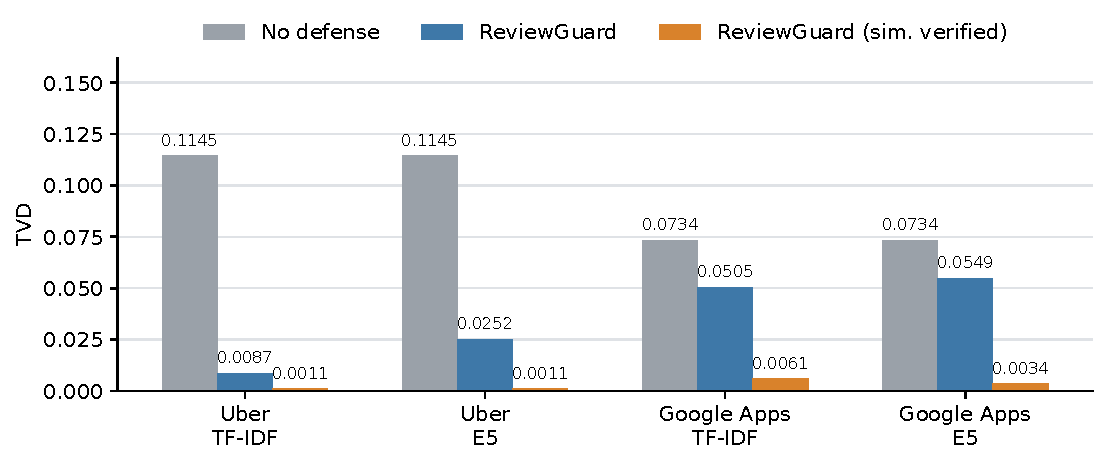
\includegraphics[width=0.98\linewidth]{paper_cross_dataset_representation_tvd.pdf}
\caption{Multi-stream representation comparison at 20\% attack using separate within-stream evaluations. Lower TVD is better.}
\label{fig:cross}
\end{figure}

\subsection{Ablation Study}

Table~\ref{tab:formula} removes one signal or replaces the product rule and averages TVD over the 10\%, 20\%, 30\%, and 40\% attack settings. The full product rule achieves the lowest overall mean TVD across the two streams. Its advantage is not uniform, however: on the pooled multi-app Google Apps stream, removing loss-based consistency improves mean TVD from 0.0494 to 0.0334, while the same ablation degrades Uber from 0.0111 to 0.0791. This confirms that the contribution of loss-based consistency is data-dependent rather than universally beneficial.

\begin{table}
\centering
\caption{ReviewGuard ablation averaged over 10\%, 20\%, 30\%, and 40\% attack ratios. Lower mean TVD is better.}
\label{tab:formula}
\begin{tabular}{lrrr}
\toprule
Variant & Uber & Google Apps & Overall\\
\midrule
ReviewGuard: group + loss + product & \textbf{0.0111} & 0.0494 & \textbf{0.0303}\\
ReviewGuard - group evidence & 0.0781 & 0.1010 & 0.0896\\
ReviewGuard - loss-based consistency & 0.0791 & \textbf{0.0334} & 0.0563\\
ReviewGuard - product + linear average & 0.0770 & 0.0637 & 0.0704\\
ReviewGuard - product + geometric mean & 0.0510 & 0.0539 & 0.0525\\
ReviewGuard - product + minimum rule & 0.0152 & 0.0477 & 0.0314\\
\bottomrule
\end{tabular}
\end{table}

Pearson correlations between the two reliability scores \(c_i\) and \(u_i\) are -0.177 on Uber and -0.181 on Google Apps. Feature ablation shows that low-rating and duplicate-text evidence are the most important cohort features: removing them increases Uber TVD to 0.0659 and 0.0364, respectively. In this setting, removing semantic or version evidence instead slightly improves TVD to 0.0068 and 0.0072, suggesting that the default weighting may overemphasize these supporting signals. Their marginal value is therefore data-dependent rather than uniformly positive.

\subsection{Further Analyses}

\paragraph{Attack-type analysis.}
Across the tested attack types, ReviewGuard reduces TVD from 0.0829 to 0.0167 on mixed-rating camouflage and from 0.1259 to 0.0269 on template review bombs with duplicated negative text; it obtains 0.0480 on paraphrase review bombs with semantically similar negative text while improving over no defense. Slow-drift attacks remain harder for the loss-only method, supporting the complementarity of group and loss evidence without implying general robustness.

We additionally use a \emph{partially adaptive mixed attack} as a harder stress test at 20\% injection. Its 1,800 reviews have no duplicate normalized text, span six days and are not concentrated in a single hour, sample the three most frequent observed app versions, mix 50\% 1-star, 30\% 2-star, 10\% 3-star, and 10\% 4-star ratings, and cover cancellation, charge/refund, crash/login, and map/pickup complaints. Under base weighting, TVD decreases from 0.1046 without defense to 0.0430 (a 58.9\% reduction); injected reviews receive median and mean contribution weights of 0.294 and 0.293. The reduction is weaker than in the more conspicuous duplicated-template and mixed-rating cases, but shows mitigation when coordinated evidence is less concentrated. This harder stress test does not constitute a broad deployment guarantee.

\paragraph{Natural low-rating burst diagnostic.}

We conduct a false-positive diagnostic on the non-injected Uber analysis split to test whether ReviewGuard simply downweights temporally concentrated low-rating reviews. This is not a ground-truth spam-detection experiment: naturally occurring low-rating bursts are not verified clean labels, and the diagnostic does not establish whether any individual review is spam. Using no attack labels, we select hourly buckets whose count of 1--2-star reviews exceeds the mean plus two standard deviations and is at least five, then retain only buckets with maximum normalized-text duplicate share at most 0.30. This yields 23 text-diverse natural-burst buckets containing 227 reviews. We run base ReviewGuard weights without simulated verified-sample calibration and compare their weight distribution with the injected rows of the fixed 20\% attack stream.

Natural low-rating bursts receive some reduction because they are temporally concentrated, but their weights remain substantially higher than injected coordinated attacks: their median and mean weights are 0.648 and 0.597, versus 0.176 and 0.272 for all 1,800 injected rows. Only 14.1\% of natural-burst reviews have \(w<0.3\), compared with 67.4\% of injected rows. This diagnostic suggests that ReviewGuard does not merely penalize negative review bursts; the strongest downweighting occurs when low-rating concentration is accompanied by duplicate, semantic, rating, version, or cohort evidence. The paraphrase-only attack is a closer case (median weight 0.602), so this diagnostic should be interpreted as a comparison with the aggregate coordinated stream rather than evidence of perfect separation for every attack type.

\begin{center}
\small
\refstepcounter{table}
\textbf{Table~\thetable.} False-positive diagnostic on Uber natural low-rating bursts. Natural bursts are selected from the non-injected analysis split using time-bucket counts and an exact-duplicate diversity filter. Weights are computed by ReviewGuard in base mode without verified-sample calibration.
\label{tab:natural_burst_false_positive}
\medskip
\resizebox{\linewidth}{!}{%
\begin{tabular}{lrrrrrrr}
\toprule
Group & \#Reviews & \#Buckets & Max dup. share & Median \(w\) & Mean \(w\) & \(\%\,w<0.3\) & \(\%\,w<0.5\)\\
\midrule
Normal low-rating reviews & 1,974 & -- & 0.004 & 0.779 & 0.639 & 18.4 & 22.4\\
Natural low-rating burst & 227 & 23 & 0.009 & 0.648 & 0.597 & 14.1 & 18.9\\
Injected attacks (aggregate) & 1,800 & -- & 0.046 & 0.176 & 0.272 & 67.4 & 73.8\\
\bottomrule
\end{tabular}
}
\end{center}

\paragraph{Oracle diagnostic.}
A non-deployable oracle sweep over fixed cohort-feature weight vectors indicates that the default vector is not globally optimal, suggesting room for future automatic weighting; because this diagnostic uses the evaluation reference, it is not used for deployment claims.



\subsection{Scaling Evaluation}

Beyond the 12,000-review Uber and 12,495-review Google Apps datasets, we construct 25k, 50k, and 100k replayed review pools while preserving text, ratings, and versions. At the 100k-pool setting, ReviewGuard reduces TVD from 0.1139 without filtering to 0.0074.

\subsection{Case Study}

\paragraph{Review-level examples.}
On the fixed 20\% stream, the injected template instance ``Uber is unusable after the old update. Driver cancels and I still get charged'' (row \texttt{attack\_279}, timestamp 2024-12-11 05:19:20, version \texttt{4.532.10001}) receives weights of 1.000 without defense and 0.191, 0.952, and 0.182 from group-only, loss-only, and ReviewGuard weighting. Thus, group evidence penalizes an injected review retained by loss-only weighting. The non-injected review ``So far my experience with Uber has been awesome'' (row \texttt{real\_6402}) receives 0.967, 0.968, and 0.936, retaining most of its contribution. Figure~\ref{fig:reviewguard_workflow} contains only the method flow.

\section{Conclusion}

ReviewGuard recovers rating-derived sentiment proportions by combining group and loss reliability while retaining every review record. Injection experiments show lower TVD across attack ratios and streams, with further gains from calibration using a simulated rather than human-verified clean sample. Attack-type, stress-test, false-positive, scaling, and ablation analyses delimit these results. Future work can extend the formulation to joint sentiment-topic recovery.

\bibliographystyle{splncs04}
\bibliography{references}
\end{document}
